\chapter{Introduction}

Durant ce projet, notre groupe a pu beaucoup apprendre tant sur le plan pratique
que sur celui du travail de groupe. Tout d'abord, ce projet étant bien plus
orienté que celui du S2, il est clair que nous ne partions d'absolument rien en
termes de connaissance sur les réseaux de neurones. De plus, la majorité de
notre groupe (3 personnes sur 4) n'avait même encore jamais codé en C.

Par conséquent, une longue phase de documentation tant sur la théorie de l'OCR
que sur son implémentation en C et sur le langage en lui-même a été nécessaire.
Ceci a légèrement retardé la phase initiale de développement des tâches
individuelles, mais fut rapidement rattrapé puisque chacun a su atteindre les
objectifs pour au final obtenir un OCR fonctionnel, capable de reconnaître
plusieurs polices d'écriture dans de nombreuses conditions d'images initiales
(penchée, avec du bruit, en couleur, etc.).

Nous avons également pris le temps de s'expliquer nos parties respectives afin
que chacun possède une vue d'ensemble du projet final.

Nous exposerons donc dans ce rapport la réalisation du projet en tant que groupe
ainsi qu'en tant qu'individu sur ces deux derniers mois. Nous vous souhaitons
une bonne lecture, et vous remercions d'avance pour le temps que vous accorderez
à la lecture de ce rapport de projet

\begin{figure}
    \centering
    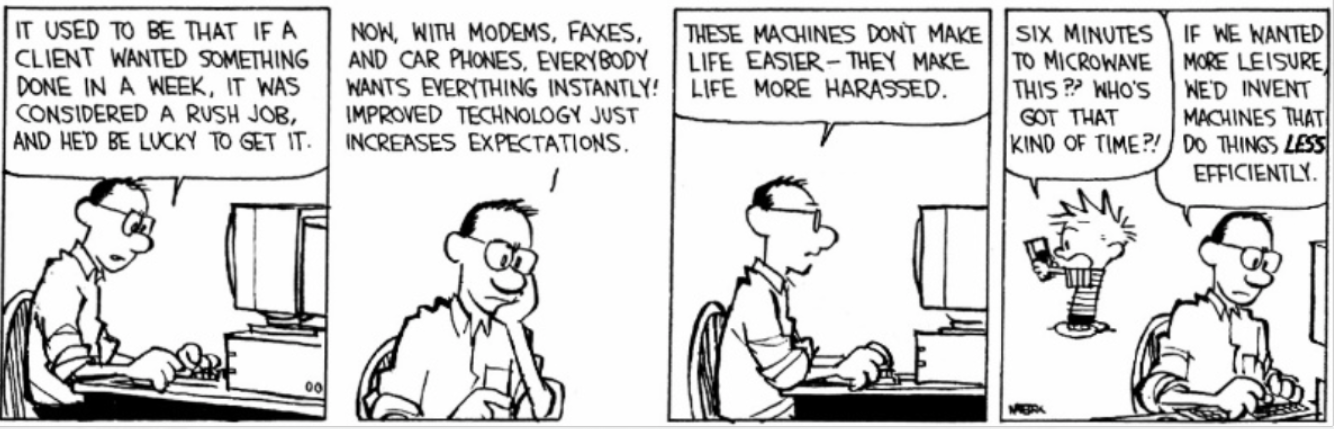
\includegraphics[width=1.1\textwidth]{calvin2}
    \caption*{\textit{Calvin and Hobbes}, Bill Watterson}
\end{figure}

\chapter{Présentation de l'équipe}

\section{Thibault Allançon (Chef de projet)}

Prolotiste jusqu’au-boutiste et peu pacifiste. Heureusement pour lui, Thibault
est plus à l'aise en C qu'en rimes. D'ailleurs, il adore parler de lui à la 3ème
personne, ce qui le rend entièrement apte à diriger ce projet de manière
optimale (la preuve sera laissée comme exercice au lecteur).

\section{Timothé Helme-Guizon}

Amateur d'animés, jeux vidéo, et programmation, ce jeune homme semblait paré à
attaquer le projet d'OCR. Malheureusement, sa compréhension du réseau de
neurones fut impossible, car on ne peut comprendre cette notion en ne possédant
qu'un seul et unique neurone.

\newpage

\section{Quentin Le Helloco}

Autostoppeur intergalactique, il s'intéresse à l'intelligence artificielle afin
de faire de Skynet une réalité. L'OCR semble être un bon moyen de commencer sa
destruction de l'humanité (lorsqu'il n’est n'est pas trop occupé à jouer au
football avec des hot-wheels).

\section{Adrian Rivoire-Galkiewicz}

Maître magicien à ses heures perdues, il a déjà réussi à faire disparaître le
nez d’un enfant. On le cherche toujours (l'enfant, pas le nez). Devenu pro dans
l’art de la manipulation, il a réussi à faire croire pendant 18 années que son
vrai nom était Adri\textbf{A}n alors que tout le monde sait qu’il n’existe que
la forme avec un \textbf{E}.  La légende raconte même qu'il est parvenu à
infiltrer l'EPITA.

\chapter{Répartition des tâches}

Les rôles des membres ont été répartis selon les souhaits de chacun. Les
différentes parties du projet ont ainsi été assignées assez rapidement, et tout
le monde a été satisfait de son rôle dans ce projet.

Nous avons également pris le temps de s'expliquer entre nous nos parties
respectives afin d'être sûr que chacun ait pu avoir un apprentissage pratique
comme théorique du projet dans sa globalité.

\vspace{2em}

\begin{center}
    \begin{tabular}{@{} l *4c @{}}
        \toprule
        \multicolumn{1}{c}{} &
            \textbf{Thibault} & \textbf{Timothé}  &
            \textbf{Quentin} & \textbf{Adrian} \\
        \midrule
        Réseau de neurones & R & & S & \\
        Suppression couleurs & & & & R \\
        Pré-traitement & S & S & R & \\
        Segmentation & S & R & & \\
        Interface & & & S & R \\
        \bottomrule
        \multicolumn{4}{l}{\footnotesize R = responsable, S = suppléant}\\
    \end{tabular}
\end{center}

\begin{center}
    \begin{tabular}{@{} l *4c @{}}
        \toprule
        \multicolumn{1}{c}{} & \textbf{Soutenance 1}  & \textbf{Soutenance 2} \\
        \midrule
        \textbf{Réseau de neurones} \\
        Structure du réseau & 80\% & 100\% \\
        Apprentissage & 60\% & 100\% \\
        Jeu de données & 45\% & 100\% \\\\
        \textbf{Pré-traitement} \\
        Suppression des couleurs & 90\% & 100\% \\
        Formatage de l'image & 0\% & 100\% \\\\
        \textbf{Segmentation} & 55\% & 100\% \\\\
        \textbf{Interface} & 30\% & 100\% \\
        \bottomrule
    \end{tabular}
\end{center}

\vspace{2em}

Vu notre avancement dès la première soutenance, nous avons pris le temps d'aller
plus loin pour la soutenance finale et de développer plusieurs bonus notamment
sur le pré-traitement de l'image (avec le redressement de l'image, ou encore la
suppression du bruit).
